%!TEX root = principal.tex
\section{Contadores}

Contadores crescentes e decrescentes. Tem o nome \%Cxx e conta com dois valores numéricos: \%Cxx.V, o valor de contagem e \%Cxx.P, o valor de preset. Na implementação do classicladder, o contador pode contar de 0 a 9999. O contador tem as seguintes entradas que modificam o valor de contagem V:
\begin{description}
	\item[R -- reset] leva o contador para 0 quando acionado.
	\item[P -- preset] leva o contador para o valor de preset quando acionado.
	\item[U -- up] incrementa o contador na subida.
	\item[D -- down] decrementa o contador na subida.
\end{description}

O contador tem as seguintes saídas:
\begin{description}
	\item[D -- done] acionado quando a contagem alcança o valor de preset (\%Cxx.V = \%Cxx.P).
	\item[E -- empty] acionado quando o contador está em zero e é decrementado (V vai para 9999). Também chamado de underflow.
	\item[F -- overflow] acionado quando o contador está em 9999 e é incrementado (V vai para 0).
\end{description}

As saídas também são disponíveis como variáveis, no formato \%Cxx.X, onde xx é o número do contador e X a variável (V, P, D, E ou F). O limite de contagem pode ser resolvido com o uso destas variáveis. Por exemplo, pode-se fazer um contador que conta até 34357 da forma mostrada na figura \ref{fig:cl_grande_contador}.
\begin{figure}[hbt]
	\centering
	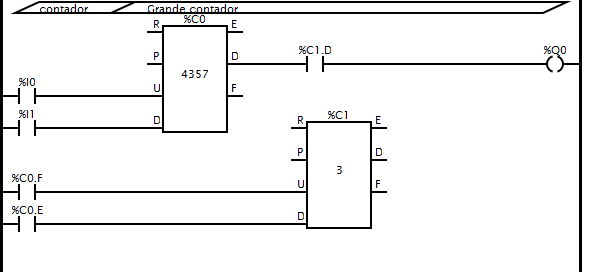
\includegraphics[width=\textwidth]{figuras/cl_grande_contador}
	\caption{Contador com preset de 34357 feito com dois contadores.}
	\label{fig:cl_grande_contador}
\end{figure}

\subsection{Acesso às variáveis}

As variáveis do contador, assim como outras variáveis numéricas, podem ser lidas ou definidas usando os blocos COMPARE ou OPERATE.

O bloco COMPARE retorna um valor booleano (acionado ou não acionado) definido por uma expressão matemática. Esta expressao pode conter:
\begin{itemize}
\item variáveis numéricas: \%W0, \%W3 ou símbolos definidos;
\item operadores matemáticos padrões, $+$, $-$, $*$, $/$, \^{} (potência), \% (módulo);
\item comparações, =, <, >, <=, >=, <> (diferente);
\item operadores lógicos, $\&$ (and), $|$ (or);
\item Funções: ABS (valor absoluta de um valor), MOY (média, em francês)/AVG (média de valores, separados por vírgula).
\end{itemize}

O bloco OPERATE é posicionado como uma bobina e recebe uma equação da forma: <variável>=valor. Se acionado acionada, como uma bobina, faz com que a variável receba o valor descrito.

Pode-se, por exemplo, definir que, quando o contador 2 contar 5, o seu valor de preset mude para 12, como mostra a figura \ref{fig:cl_contador_variaveis}.
\begin{figure}[hbt]
	\centering
	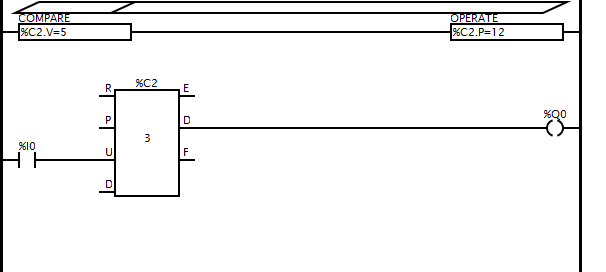
\includegraphics[width=\textwidth]{figuras/cl_contador_variaveis}
	\caption{Contador tendo seu valor de preset mudado por um bloco OPERATE.}
	\label{fig:cl_contador_variaveis}
\end{figure}

\section{Temporizadores (timers)}
O timer definido no padrão IEC61131, seguido pelo classicladder, pode ser de 3 tipos: TON, TOF ou TP. A figura \ref{fig:cl_timers} mostra um exemplo de cada um destes tipos.
\begin{figure}[hbt]
	\centering
	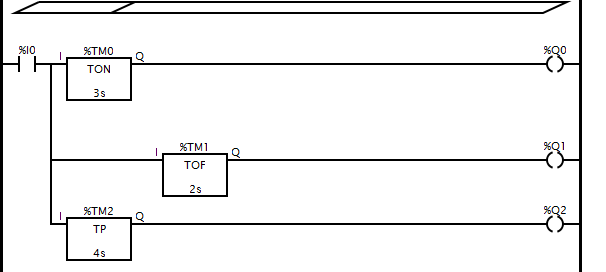
\includegraphics[width=\textwidth]{figuras/cl_timers}
	\caption{Timers TON, TOFF e TP.}
	\label{fig:cl_timers}
\end{figure}

O temporizador tipo TON causa um atraso no tempo de subida do sinal. O TOF causa um atraso no tempo de descida do sinal. O TP causa um pulso do tempo determinado iniciado pela subida do sinal de entrada. Isto pode ser visto na figura \ref{fig:tempoTimers}.
\begin{figure}[hbt]
	\centering
	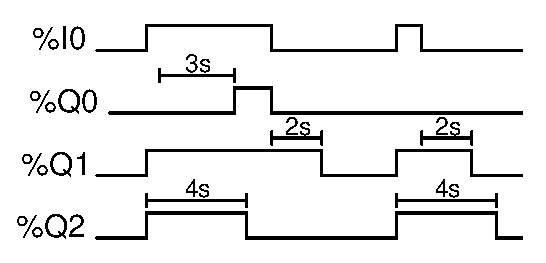
\includegraphics[scale=0.6]{figuras/tempoTimers}
	\caption{Diagrama temporal com os sinais em relação ao ladder da figura \ref{fig:cl_timers}.}
	\label{fig:tempoTimers}
\end{figure}